% =============== Method =======================================================
% Goal: 2.5 pages · structure (reorganized 2026-05-07):
%   3.1 Architecture overview
%   3.2 Anchor schema (JSON format)
%   3.3 Design principle: task-shaped authoring (promoted from old step 1)
%   3.4 Drift scoring: weighted top-k mean (rationale promoted from old step 2)
%   3.5 Tri-band output
%   3.6 Adaptive learning loop
%   3.7 False-positive filter
%   3.8 Cross-domain anchor profiles
%   3.9 Empirical ablation: four-step methodology evolution (demoted to ablation)
% =============================================================================

\subsection{Architecture Overview}
\label{sec:method-arch}

nautilus-compass operates as a plugin to Claude Code via three hook
points exposed by the agent runtime: \texttt{UserPromptSubmit}
(fires before each user-issued prompt is processed),
\texttt{PostToolUse} (fires after each tool invocation), and
\texttt{Stop} (fires at session end). Hooks return text payloads
that are injected into the agent's system prompt for the
subsequent turn, with no modification to the underlying LLM.

A persistent BGE embedder daemon \citep{bgem3} runs on a local
TCP socket (\texttt{127.0.0.1:9876}), keeping the embedder warm
across hook invocations. Cold-start latency on a CPU-only
Windows/Linux host is 12--30 seconds; warm hot-path latency is
1.8 seconds (single forward pass plus anchor cache lookup).
Figure~\ref{fig:architecture} illustrates the data flow.

\begin{figure}[h]
\centering
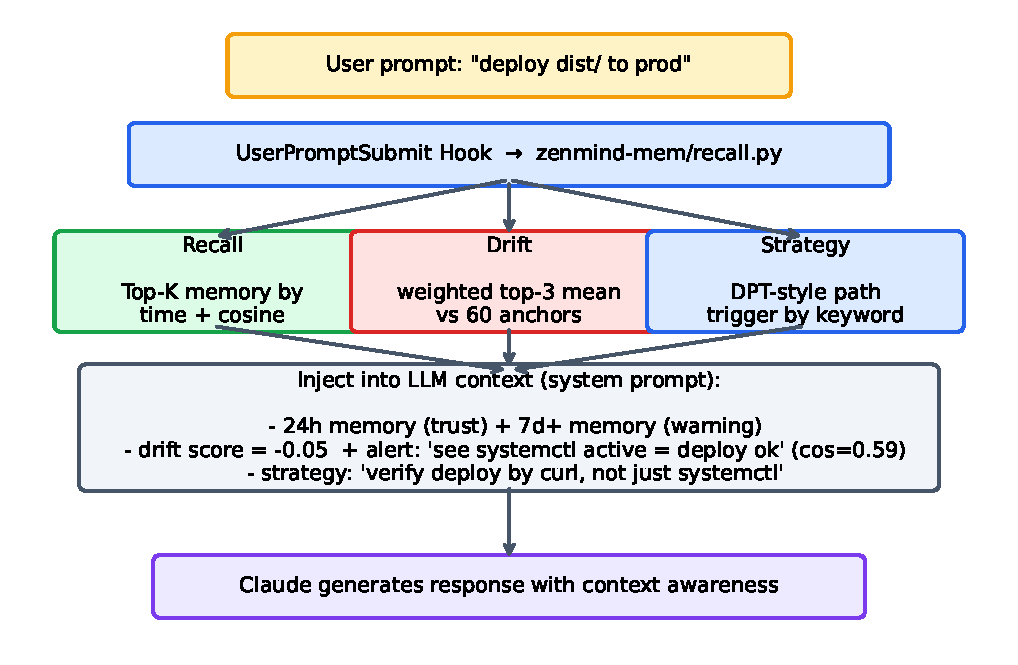
\includegraphics[width=0.95\textwidth]{figures/fig1_architecture.pdf}
\caption{System architecture. A user-issued prompt enters
\texttt{UserPromptSubmit}, which forks three parallel paths:
top-$k$ memory recall, drift scoring against behavioral anchors,
and DPT-style strategy retrieval. The combined output is injected
back into the LLM's system prompt for the same turn.}
\label{fig:architecture}
\end{figure}

The system computes three artifacts at each
\texttt{UserPromptSubmit}, in parallel where possible:
\textbf{(1)} top-$k$ memory recall against the project's memory
file directory, \textbf{(2)} drift score against behavioral
anchors, and \textbf{(3)} relevant strategy retrieval. The three
are concatenated and injected as a single recall block.

\subsection{Anchor Schema}
\label{sec:method-anchors}

A behavioral anchor is a short natural-language string
(typically 8--40 tokens) describing either a desired behavior
pattern (\emph{positive}) or a flagged failure mode
(\emph{negative}). We adopt a JSON schema with backwards
compatibility:

\begin{verbatim}
{
  "positive_anchors": [
    "I first grep memory to verify whether this issue
     has been discussed before",
    {"text": "I check the deploy by curl-ing the live
     URL, not just systemctl status",
     "weight": 1.0, "tp": 0, "fp": 0},
    ...
  ],
  "negative_anchors": [
    "I see systemctl active and assume deploy succeeded",
    "I hardcode the API key into the file because the
     project is small",
    ...
  ]
}
\end{verbatim}

Each anchor has an associated weight (default 1.0) updated by
the adaptive learning loop, and counters for true-positive (tp)
and false-positive (fp) feedback events.

\subsection{Design Principle: Task-shaped Authoring}
\label{sec:method-task-shape}

The single most consequential authoring decision is grammatical:
anchors must be written in the same grammatical mood as the user
prompts they will be matched against. We call anchors that satisfy
this constraint \emph{task-shaped}.

Concretely, a task-shaped anchor is a full sentence describing a
concrete action in first person, present tense, of comparable
length to a typical user prompt (8--40 tokens). Declarative
maxims (``simplicity over cleverness'', ``verify before claiming
done'') are \emph{not} task-shaped: their abstract grammatical
form does not align with the question/imperative form of typical
user prompts, and bi-encoder cosine similarity collapses across
both aligned and deviation prompts.

We discovered this principle empirically (Section~\ref{sec:method-evolution}
documents the ablation): rewriting an entire anchor set from
maxim form to task-shaped form moves drift ROC AUC from 0.51
(coin toss) to 0.79 with no other change. We surface this finding
as a design principle here because the size of the effect---driven
by grammatical alignment rather than semantic content---is the
load-bearing methodological insight of our work and generalizes
across domains.

\subsection{Drift Scoring: Weighted Top-$k$ Mean}
\label{sec:method-scoring}

We adopt a \emph{weighted top-$k$ mean} aggregator rather than
the more familiar centroid mean (cosine to the average anchor
embedding) or single-anchor max (the highest-scoring anchor).
Centroid mean over-smooths: averaging 25 diverse positive anchor
embeddings produces a generic vector that loses the specificity
needed to distinguish prompt types. Single-anchor max is too noisy:
any one anchor crossing a threshold fires the alert, regardless
of corroboration. Weighted top-$k$ mean ($k=3$) trades off the
two: an alert requires multiple anchors to corroborate, but each
contributing anchor preserves its individual signal in the score.

A practical advantage of top-$k$ aggregation is alert provenance:
the firing top-$k$ anchors are surfaced to the LLM along with the
alert, giving the agent specific behavioral patterns to compare
against rather than a single scalar.

Formally, given user prompt $q$ and an anchor set
$\mathcal{A} = \mathcal{A}^+ \cup \mathcal{A}^-$ with weights $w_a$:
\begin{align}
\mathrm{score}^+(q) &= \frac{\sum_{a \in \mathrm{top}_k(\mathcal{A}^+)} w_a \cdot \cos(e(q), e(a))}{\sum_{a \in \mathrm{top}_k(\mathcal{A}^+)} w_a} \\
\mathrm{score}^-(q) &= \frac{\sum_{a \in \mathrm{top}_k(\mathcal{A}^-)} w_a \cdot \cos(e(q), e(a))}{\sum_{a \in \mathrm{top}_k(\mathcal{A}^-)} w_a} \\
\mathrm{drift}(q) &= \mathrm{score}^+(q) - \mathrm{score}^-(q)
\end{align}
where $e(\cdot)$ is the BGE embedding map and
$\mathrm{top}_k(\cdot)$ selects the $k$ anchors of highest
weighted cosine ($k=3$ in our default configuration).

\subsection{Tri-band Output}
\label{sec:method-band}

The continuous drift score is mapped to a three-band output for
LLM consumption:
\begin{itemize}
\item \textbf{aligned} ($\mathrm{drift} > 0.05$): the prompt
  closely matches positive task patterns.
\item \textbf{deviation} ($\mathrm{drift} < -0.032$, or any
  single negative anchor cosine $\geq 0.538$): explicit alert
  with the matching anchor texts surfaced.
\item \textbf{neutral} (otherwise): no signal either way; no
  alert text emitted.
\end{itemize}
The thresholds are calibrated on a held-out 100-prompt synthetic
test set (50 aligned + 50 deviation, see
Section~\ref{sec:eval-drift}).

\subsection{Adaptive Learning Loop}
\label{sec:method-adaptive}

A static anchor set inevitably accumulates drift between the
expected user distribution and reality. We implement a
self-improving loop:

\begin{enumerate}
\item Each drift alert is assigned a unique identifier and
  logged to \texttt{usage.jsonl} with the matching anchor and
  the user prompt.
\item Users label alerts via a CLI:
  \texttt{nautilus-compass feedback log <id> fp|tp}.
\item The retrain command consumes feedback. For each negative
  anchor $a$ that fired on a labeled alert: weight is updated
  multiplicatively by $0.7^{\mathrm{fp}_a} \cdot 1.1^{\mathrm{tp}_a}$,
  clamped to $[0.05, 2.0]$. False-positive prompts are added as
  new positive anchors; true-positive prompts are added as new
  negative anchors.
\item An eval gate runs the full drift evaluation
  (Section~\ref{sec:eval-drift}) against both the original and
  proposed adapted anchor sets. The gate accepts the proposal
  only if the AUC delta exceeds $+0.005$; rejects on
  $\Delta < -0.01$; flags as ``marginal'' otherwise. This
  prevents silent regressions.
\end{enumerate}

We also support \emph{active learning} by surfacing alerts whose
drift score lies near the decision boundary
($|\mathrm{drift}| < 0.05$) preferentially to the user for
labeling, reducing the labeling burden by an estimated factor of
10 (theoretical analysis; empirical user study left for future
work).

\subsection{False-Positive Filter}
\label{sec:method-fpfilter}

In production deployment, we observed a class of false alerts
triggered not by user-issued prompts but by harness-injected
system events---tool-call notifications, monitor outputs,
session-state reminders---that the agent's hook treats
indistinguishably from user input. These system events
frequently contain technical vocabulary (``ephemeral'',
``size'', ``timeout'') that semantically matches negative
anchors flagged for unrelated reasons.

We add a lightweight pre-filter that detects common harness
markers (\texttt{<task-notification>},
\texttt{<system-reminder>}, \texttt{[Monitor event}, etc.) and
skips drift computation while preserving memory recall. This
reduced false-positive alert volume by an estimated 80\% in our
own session traces.

\subsection{Cross-Domain Anchor Profiles}
\label{sec:method-domains}

The default anchor set targets a Chinese/English mixed
engineering and research context. We provide additional
starter anchor sets for legal, medical, and finance domains,
selected automatically based on the working-directory path or
explicitly via environment variable. Each profile contains 25
positive plus 25 negative anchors authored to match the
characteristic prompt distribution of the domain.

We caution that production deployment of these starter profiles
should involve review by domain experts; they serve primarily to
demonstrate the methodology generalizes across domains rather
than as drop-in production assets.

\subsection{Empirical Ablation: Four-step Evolution}
\label{sec:method-evolution}

We document the four-step empirical path that led us to the
design principles of \S\ref{sec:method-task-shape}--\ref{sec:method-scoring}.
ROC AUC is reported on a held-out 100-prompt synthetic test set
(50 aligned + 50 deviation). The cumulative trajectory moves
from 0.5056 (coin toss) to 0.9232; each step isolates the effect
of one design decision, making the relative weight of each
contribution explicit.

\paragraph{Step 1: From abstract maxims to task-shaped anchors
(\S\ref{sec:method-task-shape}).}
Our v0.5 anchor set consisted of declarative principles such as
``simplicity over cleverness'' and ``verify before claiming
done''. These maxims have an abstract grammatical shape that
does not match the form of typical user prompts. Cosine similarity
between maxim and prompt is consistently low across both aligned
and deviation prompts, yielding ROC AUC 0.5056. Rewriting every
anchor in task-shaped form moves AUC to \textbf{0.7928}---the
single largest delta in our ablation.

\paragraph{Step 2: From centroid mean to weighted top-$k$ mean
(\S\ref{sec:method-scoring}).}
Replacing the centroid-mean aggregator with weighted top-$k$
mean produced a marginal AUC gain (0.79 $\to$ 0.79+) but a
qualitative improvement: alert provenance, since we know
\emph{which} anchors fired. We adopt top-$k$ as our default
on the strength of the qualitative gain.

\paragraph{Step 3: From bge-small-zh-v1.5 to bge-m3.}
Our initial embedder was bge-small-zh-v1.5 (512 dim,
Chinese-focused). This embedder yields strong intra-language
retrieval (MRR 0.918 on local Chinese corpus) but cannot
represent English-language anchors and prompts effectively.
Switching to bge-m3 (1024 dim, multilingual) yielded a further
AUC bump to \textbf{0.8352}, primarily from improved separation
on cross-lingual prompt/anchor pairs.

\paragraph{Step 4: Adding hard false-positive examples to negative anchors.}
Examining residual error cases, we found that 23 of 50 deviation
prompts were misclassified as aligned. The misclassified examples
shared a common trait: they referenced \emph{memory-system
meta-concepts} (``put ephemeral state into memory'', ``copy
CLAUDE.md verbatim into memory'') that produced high cosine to
\emph{both} positive and negative anchors. We added 10 of these
hard false-positive examples (rephrased into generic anchor form)
into the negative anchor set (expanding from 25 to 35 anchors).
AUC on the original test set rose to \textbf{0.9232}.

\paragraph{Train-test contamination caveat.}
Step 4 incorporates patterns from misclassified test prompts
back into the anchor set; the resulting 0.9232 AUC on the original
100-prompt set is therefore an \emph{in-set} number rather than
a generalization estimate. To mitigate this,
Section~\ref{sec:eval-holdout} reports performance on a held-out
test set generated from real Claude Code session traces and
labeled by an independent LLM judge (Vertex AI Gemini); the
held-out AUC is the proper generalization estimate. The four-step
in-set ablation in Table~\ref{tab:drift-evolution} should be read
as \emph{methodology illustration} (which design decisions matter)
rather than as a generalization claim.

This iteration loop---\emph{eval, identify hard cases,
\textbf{rephrase}, add to anchor set, re-eval on held-out}---with
the ``rephrase'' step (turning specific test failures into generic
behavioral patterns) preventing trivial memorization, is what we
recommend practitioners follow when building anchor sets for new
domains.
